\documentclass[12pt,a4paper]{article}
\pdfminorversion=7

% ----- PACKAGES -----
\usepackage[utf8]{inputenc}
\usepackage{graphicx}
\usepackage{geometry}
\usepackage{setspace}
\usepackage{hyperref}
\usepackage{fancyhdr}
\usepackage{titlesec}
\usepackage{booktabs}
\usepackage{multirow}
\usepackage{pgfplots}
\usepgfplotslibrary{groupplots}
\pgfplotsset{compat=1.18}
\usepackage[maxbibnames=3,minbibnames=1,maxcitenames=2,mincitenames=1,style=numeric-comp,backend=biber]{biblatex}
\addbibresource{references.bib}

\geometry{margin=1in}
\setstretch{1.2}
\setlength{\headheight}{14.5pt}
\pagestyle{fancy}
\fancyhf{}
\rhead{Project Report}
\lhead{\leftmark}
\rfoot{Page \thepage}

\title{
    \textbf{Advanced Information Retrieval}\\[0.2cm]
    \large Fine-Tuning and Transferability in Legal Information Retrieval\\[0.2cm]
    \normalsize Group Number: 27\\[0.3cm]
    \normalsize Repository: \href{https://github.com/rhabichl/Advanced-Information-Retrieval}{rhabichl/Advanced-Information-Retrieval}\\[0.15cm]
    \normalsize Adapter: \href{https://huggingface.co/krapfi/Qwen3-Embedding-8B-Ger-Legal}{krapfi/Qwen3-Embedding-8B-Ger-Legal}\\[0.3cm]
}
\author{
    Raphael Habichler\thanks{student-id: 12419578, Role: Data Processing \& Fine-tuning} \and
    Mark Sesko\thanks{student-id: 12114879, Role: Evaluation \& Analysis} \and
    Paul Brandstätter\thanks{student-id: 12212566, Role: Dataset Preparation \& Documentation}
}
\date{\today}

\titleformat{\section}{\large\bfseries}{\thesection}{1em}{}
\titleformat{\subsection}{\normalsize\bfseries}{\thesubsection}{1em}{}

\begin{document}
\pagestyle{empty}
\pagenumbering{roman}
\maketitle
\newpage
\pagenumbering{arabic}
\pagestyle{fancy}

\section{Abstract}
This project tests whether an embedding model fine-tuned on one legal system transfers to others.
We fine-tune Qwen3-Embedding-8B \cite{qwen3embedding} on German legal query-document pairs and evaluate the baseline and fine-tuned model on German, Austrian, and Chinese legal retrieval datasets.
We report Recall@k, Precision@k, and nDCG@k.
The fine-tuned model improves retrieval on German data, but we do not observe clear transfer to Austrian or Chinese data.

\section{Introduction}
Legal information retrieval is important for searching laws and cases.
However, labeled training data is often available only for some jurisdictions.
Our research question is: Can a legal embedding model fine-tuned on German law effectively retrieve relevant documents in other jurisdictions (Austrian and Chinese law)?
If transfer works, we can build better retrieval systems in low-resource settings without collecting large new training datasets.

\section{Related Work}
GerDaLIR provides a large benchmark for German legal retrieval \cite{wrzalik-krechel-2021-gerdalir}.
LeCaRDv2 provides a benchmark for Chinese legal case retrieval \cite{li2023lecardv2}.
We build on Qwen3-Embedding-8B \cite{qwen3embedding} and evaluate transfer across datasets and languages.

\section{Experiments}
\subsection{Datasets}
We use three datasets.
German data comes from GerDaLIRSmall (test split) \cite{wrzalik-krechel-2021-gerdalir}.
Chinese data comes from LeCaRDv2 (test split) \cite{li2023lecardv2}.
Austrian data is a synthetic dataset built from Austrian legal documents where we generate queries from documents.

\subsection{Model and Fine-Tuning}
We use Qwen3-Embedding-8B \cite{qwen3embedding} as the baseline embedding model.
We fine-tune the model on German query-document pairs using a LoRA adapter (PEFT) with 8-bit quantization.
Training was done on an NVIDIA GeForce RTX 3090.
We use a contrastive ranking objective (multiple negatives) to increase similarity of matching query-document pairs and decrease similarity to other documents.

\subsection{Workflow}
We first download all datasets from Hugging Face.
We then generate embeddings for all queries and documents with our embedding generation script (XXX).
After that, we train a LoRA adapter on cleaned German query-document pairs.
Finally, we evaluate retrieval by randomly sampling 1000 queries and ranking them against the full corpus.

\subsection{Retrieval and Evaluation}
For each query, we embed the query and all candidate documents and rank documents by dot product similarity.
We report Recall@k, Precision@k, and nDCG@k for \(k \in \{1,5,10,20,50,100\}\).
For German and Chinese datasets, we evaluate on a random sample of 1000 queries.
For Austrian data, each query has one matching document, and retrieval is evaluated against the full Austrian candidate set.

\section{Results}
\subsection{German (GerDaLIRSmall)}
Fine-tuning on German improves all metrics across all \(k\), with the largest gains at larger \(k\).
This supports that the LoRA adapter learns German legal retrieval patterns.

\begin{table}[h]
\centering
\setlength{\tabcolsep}{6pt}
\renewcommand{\arraystretch}{1.15}
\begin{tabular}{llrrrrrr}
\toprule
Setup & Metric & @1 & @5 & @10 & @20 & @50 & @100 \\
\midrule
\multirow{3}{*}{Baseline} & Recall & 0.1330 & 0.2343 & 0.2826 & 0.3436 & 0.4313 & 0.5066 \\
 & Precision & 0.1500 & 0.0544 & 0.0330 & 0.0204 & 0.0103 & 0.0060 \\
 & nDCG & 0.1500 & 0.2013 & 0.2214 & 0.2442 & 0.2691 & 0.2863 \\
\midrule
\multirow{3}{*}{Fine-tuned} & Recall & 0.1445 & 0.2803 & 0.3767 & 0.4788 & 0.6350 & 0.7361 \\
 & Precision & 0.1615 & 0.0643 & 0.0434 & 0.0280 & 0.0150 & 0.0087 \\
 & nDCG & 0.1615 & 0.2260 & 0.2657 & 0.3046 & 0.3508 & 0.3748 \\
\bottomrule
\end{tabular}
\caption{German retrieval results (GerDaLIRSmall test): baseline vs fine-tuned.}
\label{tab:results-german}
\end{table}

\subsection{Austrian (synthetic)}
On Austrian data, performance is very low for both models.
We see only small changes after German fine-tuning, and the improvements are not consistent across \(k\).
This suggests that German fine-tuning does not reliably transfer to this synthetic Austrian setup.

\begin{table}[h]
\centering
\setlength{\tabcolsep}{6pt}
\renewcommand{\arraystretch}{1.15}
\begin{tabular}{llrrrrrr}
\toprule
Setup & Metric & @1 & @5 & @10 & @20 & @50 & @100 \\
\midrule
\multirow{3}{*}{Baseline} & Recall & 0.0000 & 0.0040 & 0.0060 & 0.0120 & 0.0340 & 0.0460 \\
 & Precision & 0.0000 & 0.0008 & 0.0006 & 0.0006 & 0.0007 & 0.0005 \\
 & nDCG & 0.0000 & 0.0025 & 0.0032 & 0.0047 & 0.0091 & 0.0110 \\
\midrule
\multirow{3}{*}{Fine-tuned} & Recall & 0.0000 & 0.0080 & 0.0080 & 0.0100 & 0.0280 & 0.0460 \\
 & Precision & 0.0000 & 0.0016 & 0.0008 & 0.0005 & 0.0006 & 0.0005 \\
 & nDCG & 0.0000 & 0.0043 & 0.0043 & 0.0048 & 0.0083 & 0.0112 \\
\bottomrule
\end{tabular}
\caption{Austrian retrieval results (synthetic): baseline vs fine-tuned.}
\label{tab:results-austrian}
\end{table}

\subsection{Chinese (LeCaRDv2)}
On Chinese data, the fine-tuned model is slightly worse than the baseline on most \(k\).
We do not see positive transfer from German to Chinese in this setup.
This aligns with the idea that cross-lingual and cross-jurisdiction transfer is difficult without multilingual adaptation or Chinese training data.

\begin{table}[h]
\centering
\setlength{\tabcolsep}{6pt}
\renewcommand{\arraystretch}{1.15}
\begin{tabular}{llrrrrrr}
\toprule
Setup & Metric & @1 & @5 & @10 & @20 & @50 & @100 \\
\midrule
\multirow{3}{*}{Baseline} & Recall & 0.0374 & 0.1694 & 0.2912 & 0.5018 & 0.7848 & 0.9299 \\
 & Precision & 0.8239 & 0.7585 & 0.6780 & 0.5972 & 0.3824 & 0.2275 \\
 & nDCG & 0.8239 & 0.7905 & 0.7386 & 0.6992 & 0.7778 & 0.8579 \\
\midrule
\multirow{3}{*}{Fine-tuned} & Recall & 0.0380 & 0.1597 & 0.2737 & 0.4585 & 0.7472 & 0.9118 \\
 & Precision & 0.8302 & 0.7182 & 0.6296 & 0.5472 & 0.3638 & 0.2233 \\
 & nDCG & 0.8302 & 0.7575 & 0.7013 & 0.6542 & 0.7470 & 0.8407 \\
\bottomrule
\end{tabular}
\caption{Chinese retrieval results (LeCaRDv2 test): baseline vs fine-tuned.}
\label{tab:results-chinese}
\end{table}

\newpage
\section{Conclusion}
We fine-tuned Qwen3-Embedding-8B on German legal pairs and evaluated transfer to Austrian and Chinese retrieval.
We find clear improvements on German test data.
We do not find clear improvements on Austrian or Chinese datasets, and Chinese performance slightly decreases after German fine-tuning.
Overall, our results suggest that domain and language transfer is limited in this setting, and that additional multilingual training data or adaptation methods would likely be needed.

\section*{Limitations and Risks}
Our Austrian dataset is synthetic and may not match real user queries.
Cross-language transfer may require explicit multilingual training.
Legal retrieval systems can reflect bias in training data and should not be used as a substitute for legal advice.

\appendix
\section{Visualization of Results}
Figure~\ref{fig:curves} visualizes Recall@k and nDCG@k for baseline and fine-tuned models on all three datasets.
This makes it easier to compare trends across \(k\) than tables alone.

\begin{figure}[h]
\centering

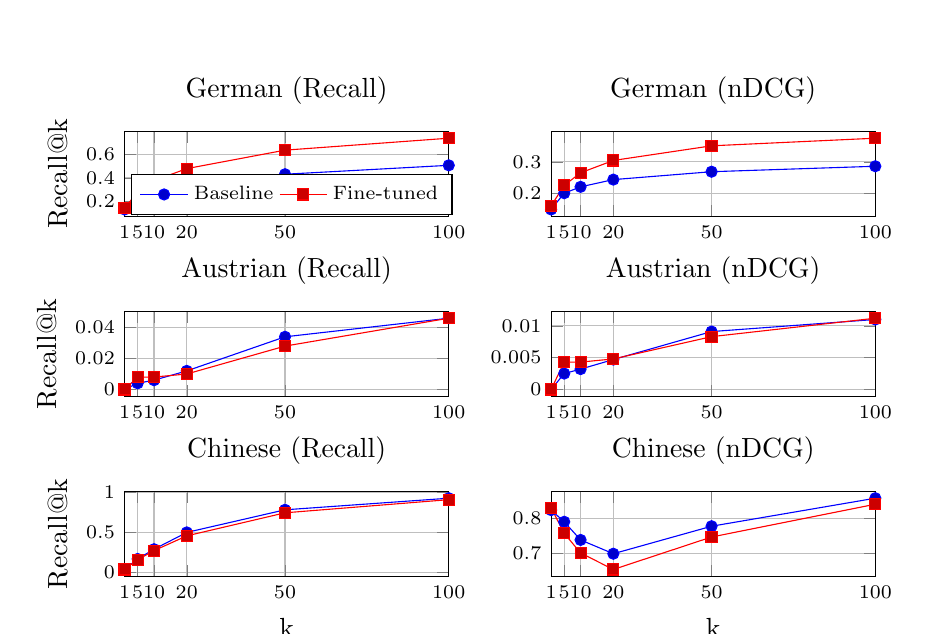
\begin{tikzpicture}
\begin{groupplot}[
  group style={group size=2 by 3, horizontal sep=1.3cm, vertical sep=1.2cm},
  width=0.47\textwidth,
  height=0.22\textwidth,
  xmin=1, xmax=100,
  xtick={1,5,10,20,50,100},
  xticklabels={1,5,10,20,50,100},
  xmode=normal,
  xlabel={},
  grid=both,
  scaled y ticks=false,
  tick label style={font=\scriptsize},
  yticklabel style={/pgf/number format/fixed, /pgf/number format/precision=3},
  title style={font=\normalsize},
  legend style={font=\scriptsize, draw=black, fill=white, at={(0.02,0.02)}, anchor=south west, legend columns=2},
  ylabel near ticks,
]

% Layout: rows = datasets (German/Austrian/Chinese), columns = metrics (Recall/nDCG)
\nextgroupplot[title={German (Recall)}, ylabel={Recall@k}]
\addplot+[mark=*] coordinates {(1,0.1330) (5,0.2343) (10,0.2826) (20,0.3436) (50,0.4313) (100,0.5066)};
\addplot+[mark=square*] coordinates {(1,0.1445) (5,0.2803) (10,0.3767) (20,0.4788) (50,0.6350) (100,0.7361)};
\legend{Baseline, Fine-tuned}

\nextgroupplot[title={German (nDCG)}, ylabel={}]
\addplot+[mark=*] coordinates {(1,0.1500) (5,0.2013) (10,0.2214) (20,0.2442) (50,0.2691) (100,0.2863)};
\addplot+[mark=square*] coordinates {(1,0.1615) (5,0.2260) (10,0.2657) (20,0.3046) (50,0.3508) (100,0.3748)};

\nextgroupplot[title={Austrian (Recall)}, ylabel={Recall@k}]
\addplot+[mark=*] coordinates {(1,0.0000) (5,0.0040) (10,0.0060) (20,0.0120) (50,0.0340) (100,0.0460)};
\addplot+[mark=square*] coordinates {(1,0.0000) (5,0.0080) (10,0.0080) (20,0.0100) (50,0.0280) (100,0.0460)};

\nextgroupplot[title={Austrian (nDCG)}, ylabel={}]
\addplot+[mark=*] coordinates {(1,0.0000) (5,0.0025) (10,0.0032) (20,0.0047) (50,0.0091) (100,0.0110)};
\addplot+[mark=square*] coordinates {(1,0.0000) (5,0.0043) (10,0.0043) (20,0.0048) (50,0.0083) (100,0.0112)};

\nextgroupplot[title={Chinese (Recall)}, xlabel={k}, ylabel={Recall@k}]
\addplot+[mark=*] coordinates {(1,0.0374) (5,0.1694) (10,0.2912) (20,0.5018) (50,0.7848) (100,0.9299)};
\addplot+[mark=square*] coordinates {(1,0.0380) (5,0.1597) (10,0.2737) (20,0.4585) (50,0.7472) (100,0.9118)};

\nextgroupplot[title={Chinese (nDCG)}, xlabel={k}, ylabel={}]
\addplot+[mark=*] coordinates {(1,0.8239) (5,0.7905) (10,0.7386) (20,0.6992) (50,0.7778) (100,0.8579)};
\addplot+[mark=square*] coordinates {(1,0.8302) (5,0.7575) (10,0.7013) (20,0.6542) (50,0.7470) (100,0.8407)};

\end{groupplot}
\end{tikzpicture}

\caption{Recall@k and nDCG@k trends for baseline vs fine-tuned across datasets.}
\label{fig:curves}
\end{figure}

\newpage
\section{Workflow Diagram}
Figure~\ref{fig:flowchart} shows the workflow from data collection to evaluation.

\begin{figure}[h]
\centering
\includegraphics[width=\textwidth]{../design-document/flowchart.pdf}
\caption{Project workflow and methodology.}
\label{fig:flowchart}
\end{figure}

\newpage
\printbibliography
\end{document}

